\documentclass[t,professionalfonts,handout, xcolor=pdftex,dvipsnames,table]{beamer}

\usepackage{pgfpages}
\usepackage{graphics}
\usepackage{graphicx}
\usepackage{amssymb, amsmath}
\usepackage{fancybox}
\usepackage{rotating}
\usepackage{color}

\font\bbb=msbm10
\def \R {\hbox{\bbb R}}
\def \E {\hbox{\bbb E}}
\def \V {\hbox{\bbb V}}
\def \P {\hbox{\bbb P}}
\def \C {\hbox{\bbb C}}

\def\MET{\mbox{${\hbox{$E$\kern-0.6em\lower-.1ex\hbox{/}}}_T$}}
\def\squark{$\tilde{q}$}                 %squark
\def\gluino{$\tilde{g}$}                  %gluino
\def\chipm{$\tilde{\chi}^{\pm}$}   %chi+/-
\def\chiz{$\tilde{\chi}^0$}              %chi0

\def\Journal#1#2#3#4{{#1} {\bf #2}, #3 (#4)}

\newcommand{\Equation}[1]{Equation (\ref{eq:#1})}
\newcommand{\Eq}[1]{Eq.\ (\ref{eq:#1})}
\newcommand{\Eqs}[2]{Eqs.\ (\ref{eq:#1}) and (\ref{eq:#2})}
\newcommand{\Eqns}[3]{Eqs.\ (\ref{eq:#1}), (\ref{eq:#2}) and (\ref{eq:#3})}
\newcommand{\Fig}[1]{Fig.\ \ref{fig:#1}}
\newcommand{\Figs}[2]{Figs.\ \ref{fig:#1} and \ref{fig:#2}}
\newcommand{\Figure}[1]{Figure\ \ref{fig:#1}}
\newcommand{\Figures}[2]{Figures\ \ref{fig:#1} to \ref{fig:#2}}
\newcommand{\Sec}[1]{Sec.~\ref{sec:#1}}

\newcommand{\barR}{\overline{\bf R}}
\newcommand{\prob}[2]{ \mbox{P} (#1 | #2)}
\newcommand{\pdf}[2]{ f (#1 | #2)}
\newcommand{\priorpdf}[1]{ \pi (#1)}
\newcommand{\prior}[1]{ \mbox{P} (#1)}
\newcommand{\like}[1]{ L (#1)}
\newcommand{\flatpri}[1]{\pi_{\rm F}(#1)}
\newcommand{\tab}{aaaaa\=}
\newcommand{\WIDTH}{8.0cm}
\newcommand{\ANGLE}{90}
\newcommand{\SIZE}{0.375\textwidth}

\newcommand{\rlambda}{\textcolor{red}{\lambda}}
\newcommand{\bkappa}{\textcolor{blue}{\kappa}}
\newcommand{\mnu}{\textcolor{magenta}{\nu}}

\usecolortheme[named=Blue]{structure}
\setbeamertemplate{navigation symbols}{}
\setbeamercovered{transparent}

%\usetheme{Warsaw}
%\useoutertheme{infolines}
\usetheme{Madrid}

\title[Contact Interactions]{Search for Contact Interactions using the Inclusive Jet Production Cross Section @ 13\,TeV}
\author[S.Beri, S. Dutt, B. Kotwal, S. Kim, H.B. Prosper]{Suman Beri \inst{1}, Suneel Dutt, Bipen Kotwal \inst{2}, Suho Kim\inst{3}, and \underline{Harrison B. Prosper} \inst{3}}
\institute[CMS]{\inst{1} Panjab University, \inst{2} Shoolini University \and \inst{3} Florida State University}

\date{\today}

\begin{document}
\maketitle

% -----------------------------------------------------------------------------------------------------------------------------------
\AtBeginSection[] % repeat outline before each new section
{
\begin{frame}
	\frametitle{Outline}
	\tableofcontents[currentsection] % highlight current section
\end{frame}
}

% -----------------------------------------------------------------------------------------------------------------------------------
\section{Introduction}
\begin{frame}

Many thanks to members of the \textcolor{blue}{Inclusive Jet $p_T$ Group}, and especially
to Engin Eren.
\bigskip

\centerline{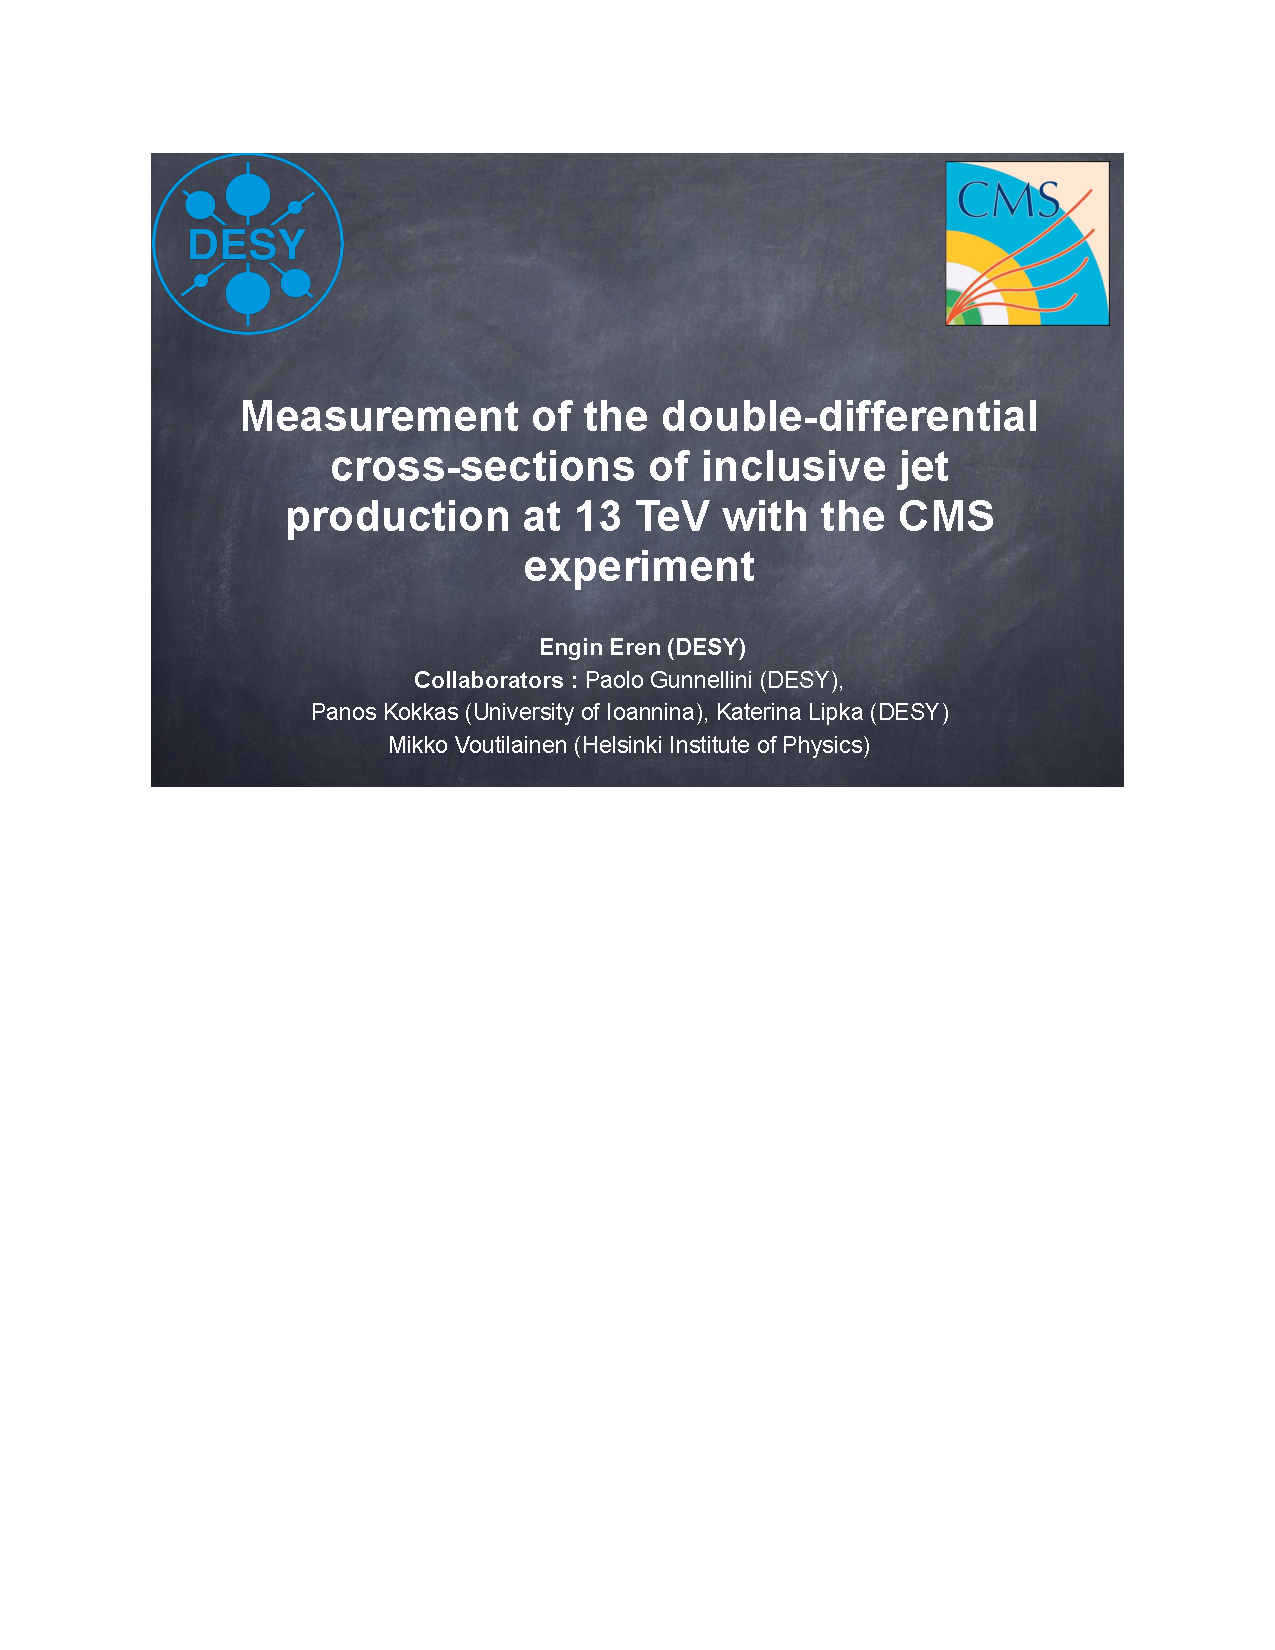
\includegraphics[width=0.8\textwidth]{figures/Engin.pdf}}

\end{frame}

%%%%%%%%%%%%%%%%%%%%%%%%%%%%%%%%%%%%%%%%%%%%%%%
\begin{frame}
\textcolor{blue}{Search for Contact Interactions}
\smallskip

Look for deviations in the high-$p_T$ tail of the inclusive jet $p_T$ spectrum 
at 13\,TeV from the predictions of QCD and
interpret deviations as potential evidence of new QCD-like interactions that cannot be resolved
at LHC energies.
\smallskip

\textcolor{blue}{Assumptions}
\begin{enumerate}
\item At LHC energies, the Lagrangian $L$ can be written as
$$L = L^{(0)}_{SM} + \frac{1}{\Lambda} L^{(1)} + \frac{1}{\Lambda^2} \textcolor{blue}{L^{(2)}} + \cdots,$$

\item with $\textcolor{blue}{L^{(2)}}$ a sum
$\textcolor{blue}{2\pi  \sum_{i=1}^6 \kappa_i \, O_i}$ over dim-6 operators $O_{1,2} \sim \bar{\psi}_L \gamma_\mu \psi_L\,\bar{\psi}_L \gamma^\mu \psi_L$,  $O_{3,4} \sim \bar{\psi}_L \gamma_\mu \psi_L\,\bar{\psi}_R \gamma^\mu \psi_R$.
$O_{5,6} \sim \bar{\psi}_R \gamma_\mu \psi_R\,\bar{\psi}_R \gamma^\mu \psi_R$ that 
describe \textcolor{blue}{contact interactions} (CI).  \textcolor{blue}{$\kappa_i$} are additional free parameters\footnote{J. Gao, Comput.Phys.Commun. 184 (2013) 2362.}.
\end{enumerate}
\end{frame}


%%%%%%%%%%%%%%%%%%%%%%%%%%%%%%%%%%%%%%%%%%%%%%%
\section{Strategy}
\begin{frame}
\textcolor{blue}{Strategy}  
\begin{enumerate}
\item
Given observed jet counts, $N_i$ in $M$ $p_T$ bins, construct a multinomial likelihood 
\begin{align*}
p(D \, |\, \rlambda, \bkappa, \nu) & = \prod_{i=1}^M \left( \frac{\sigma_i}{\sigma} \right )^{N_i},
\end{align*}
where $\rlambda \equiv 1/\Lambda^2$,  $\sigma_i$
is the predicted cross section in the $i^\text{th}$ bin, $\sigma = \sum_{i=1}^M \sigma_i$, and $\nu$ denotes the nuisance parameters. 
\item
Given a prior density $\pi(\rlambda, \bkappa, \nu) = \pi(\nu  \, | \,  \rlambda, \bkappa)  \pi(\rlambda | \bkappa) \pi(\bkappa)$, 
compute the marginal likelihood
\begin{align*}
p(D \, |\, \rlambda, \bkappa) & = \int p(D \, |\, \rlambda, \bkappa, \nu  )  \pi(\nu  \, | \,  \rlambda, \bkappa)  \, d\nu , \nonumber
\end{align*}
and then the posterior density $p(\rlambda |  D) \sim  p(D \, |\, \rlambda, \bkappa)  \pi(\rlambda | \bkappa)$
from which we estimate $\rlambda$ or set limits.
\end{enumerate}

\end{frame}

%%%%%%%%%%%%%%%%%%%%%%%%%%%%%%%%%%%%%%%%%%%%%%%%
\begin{frame}
\textcolor{blue}{Cross Section}  The cross section per $p_T$ bin can be
written as
\begin{align*}
\sigma 	& = \sigma_{QCD} \\
		& + \rlambda \sum_{i=1}^6 \bkappa_i (b_i + a_i g + a_i f)\\
		& + \rlambda^2  \sum_{i=1}^6 \bkappa_i^2 (b_i + a_i g + a_i f)\\
		& + \rlambda^2 \sum_{i=1,3,5} \bkappa_i \bkappa_{i+1} (b_{ii+1} + a_{ii+1} g + a_{ii+1} f)\\
		& + \rlambda^2  \sum_{i=1,2,5,6} \bkappa_i \bkappa_{4} (b_{i4} + a_{i4} g + a_{i4} f),
\end{align*}
where 
$f = \ln(\sqrt{k / \rlambda})$ and the \textcolor{blue}{57} coefficients are independent of $\rlambda$\footnote{J. Gao, Comput.Phys.Commun. 184 (2013) 2362.}.
\end{frame}

\begin{frame}
\textcolor{blue}{Distributions of 57 CI Coefficients}
\bigskip
 
 \centerline{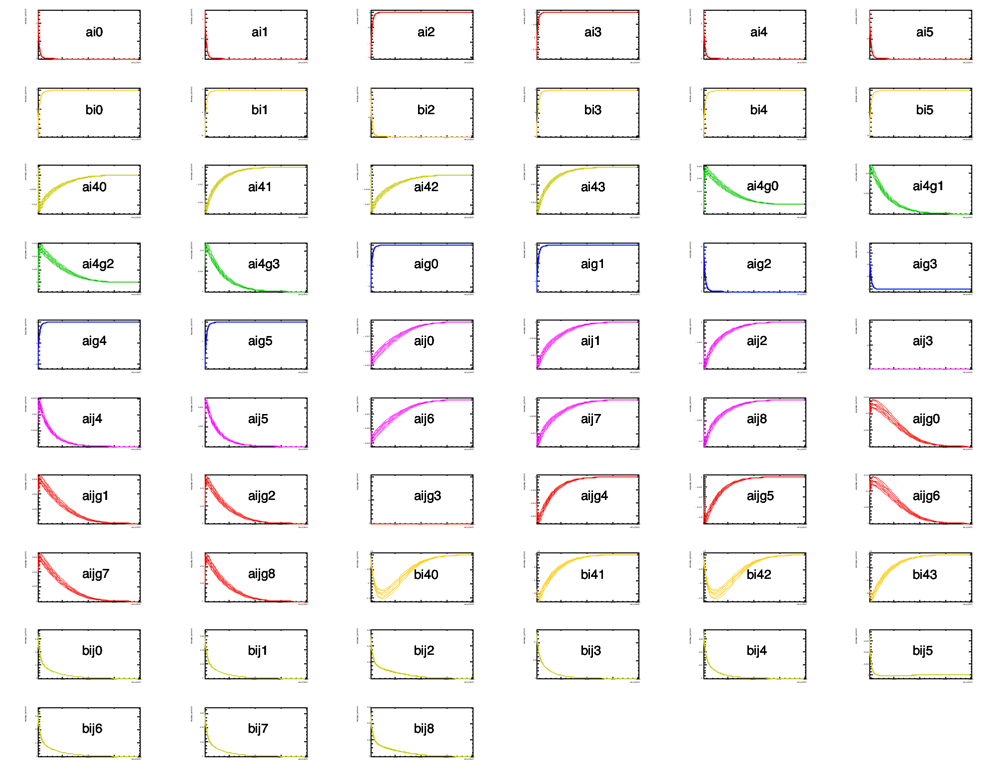
\includegraphics[width=0.8\textwidth]{coeff13TeV.png}}
\end{frame}

%%%%%%%%%%%%%%%%%%%%%%%%%%%%%%%%%%%%%%%%%%%%%%%%

\begin{frame}
The main task is modeling the prior $ \pi(\nu  \, | \,  \rlambda, \bkappa) $:
\begin{enumerate}
\item Use \textcolor{blue}{\tt hessian2replicas} in \textcolor{blue}{\tt LHAPDF6.1.6} to generate an ensemble of PDF sets for \textcolor{blue}{\tt CT14nlo} and \textcolor{blue}{\tt MMHT2014nlo68cl}. We also use
\textcolor{blue}{\tt NNPDF30\_nlo\_as\_0118\_1000}.
\item For each PDF set, and 7 combinations of renormalization and factorization scales, use 
\textcolor{blue}{\tt fastnlo\_toolkit-2.3.1pre-2411} to compute the QCD cross section and
 \textcolor{blue}{\tt CIJET1.1} to compute the 57 CI
coefficients. Do this for  each of  $M$ jet $p_{T}$ bins. 
\item Randomly select a consistent set of  CI coefficients and QCD cross sections and  randomly select 
a jet response function \textcolor{blue}{JRF}. Convolve the 58 differential distributions with the (\textcolor{blue}{JRF}). 
\item Repeat 2 and 3 a few hundred times.
\end{enumerate}
\end{frame}

%%%%%%%%%%%%%%%%%%%%%%%%%%%%%%%%%%%%%%%%%%%%%%%%

\section{Preliminary Results}
\begin{frame}
Inclusive jet spectrum at 13\,TeV (${\cal L} = 35.1\,\textrm{fb}^{-1}$) compared with a $\Lambda = 30\,\textrm{TeV}$ CI signal.

\medskip

\textcolor{blue}{Constructive interference}

\medskip

\begin{columns}[T]

\begin{column}{0.49\textwidth}
\centerline{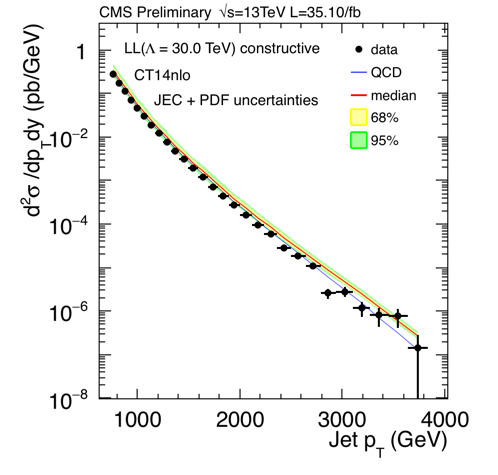
\includegraphics[width=\textwidth]{xsection_LL.png}}
\end{column}

\begin{column}{0.49\textwidth}
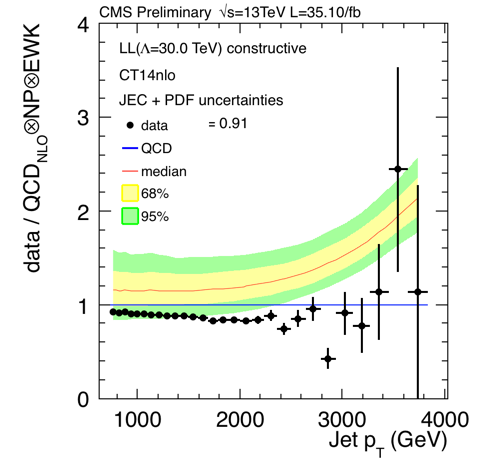
\includegraphics[width=\textwidth]{xsection_LL_ratio.png}
\end{column}

\end{columns}

\end{frame}

%%%%%%%%%%%%%%%%%%%%%%%%%%%%%%%%%%%%%%%%%%%%%%%%

\begin{frame}
Inclusive jet spectrum at 13\,TeV (${\cal L} = 35.1\,\textrm{fb}^{-1}$) compared with a $\Lambda = 30\,\textrm{TeV}$ CI signal.

\medskip

\textcolor{red}{Destructive interference}

\medskip

\begin{columns}[T]

\begin{column}{0.49\textwidth}
\centerline{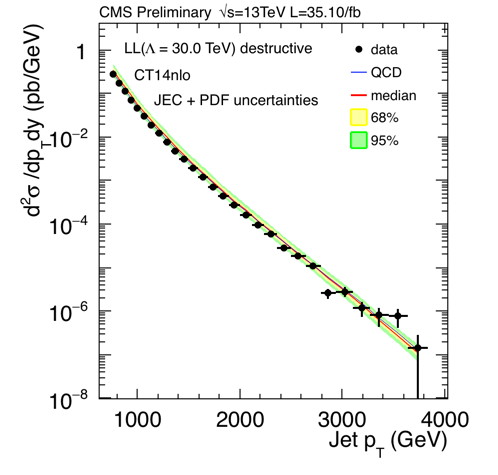
\includegraphics[width=\textwidth]{xsection_LL_d.png}}
\end{column}

\begin{column}{0.49\textwidth}
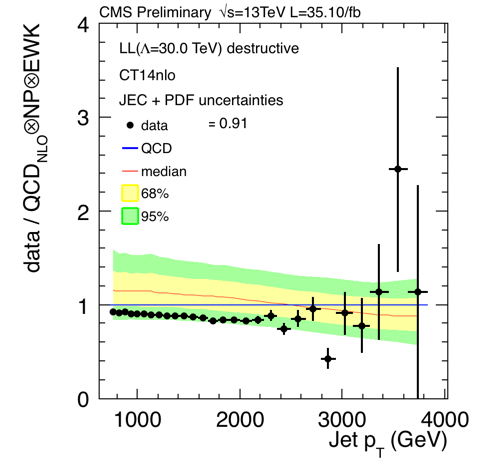
\includegraphics[width=\textwidth]{xsection_LL_ratio_d.png}
\end{column}

\end{columns}

\end{frame}

%%%%%%%%%%%%%%%%%%%%%%%%%%%%%%%%%%%%%%%%%%%%%%%%

\begin{frame}
\textcolor{blue}{Expected limits for LL CI model} 

13\,TeV (${\cal L} = 35.1\,\textrm{fb}^{-1}$)

\medskip

\begin{columns}[T]

\begin{column}{0.49\textwidth}
\centerline{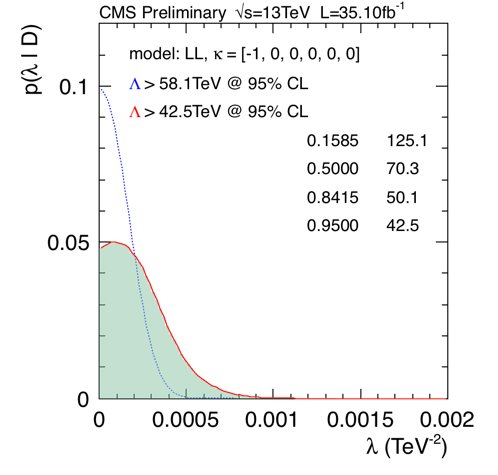
\includegraphics[width=\textwidth]{limit_c.png}}
\end{column}

\begin{column}{0.49\textwidth}
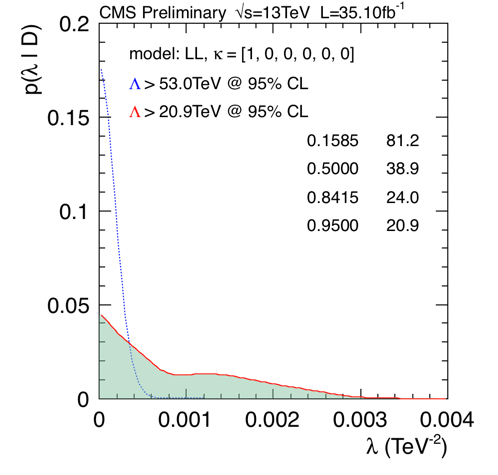
\includegraphics[width=\textwidth]{limit_d.png}
\end{column}

\end{columns}

\end{frame}

%%%%%%%%%%%%%%%%%%%%%%%%%%%%%%%%%%%%%%%%%%%%%%%%

\begin{frame}
\textcolor{blue}{Checking the Likelihood} 

13\,TeV (${\cal L} = 100\,\textrm{fb}^{-1}$) \textcolor{blue}{$\Lambda = 30\,\textrm{TeV}$}

\medskip

\begin{columns}[T]

\begin{column}{0.49\textwidth}
\centerline{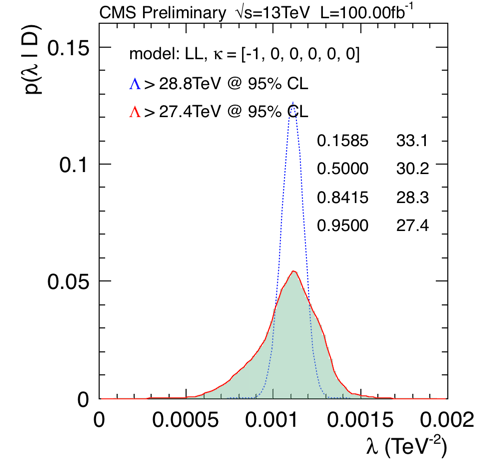
\includegraphics[width=\textwidth]{limit_LL_c_100.png}}
\end{column}

\begin{column}{0.49\textwidth}
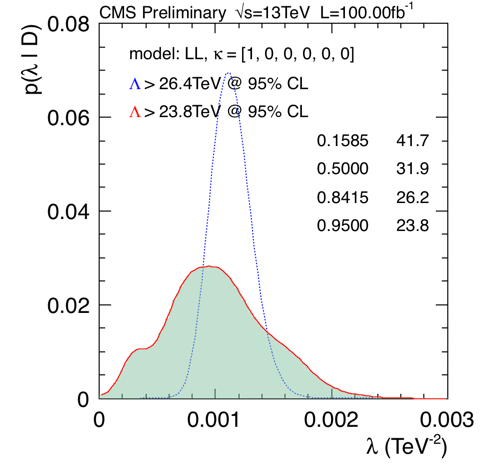
\includegraphics[width=\textwidth]{limit_LL_d_100.png}
\end{column}

\end{columns}

\end{frame}

%%%%%%%%%%%%%%%%%%%%%%%%%%%%%%%%%%%%%%%%%%%%%%%%

\section{Plans}
\begin{frame}
\textcolor{blue}{Plans}
\begin{itemize}
\item Complete analysis note and ask for an ARC
\item Check, check, check!
\item Compute expected limits for all CI models and all PDFs
\item Compute observed limit
\item Write paper
\item Publish!
\end{itemize}
\end{frame}



\end{document}